\footnotesize
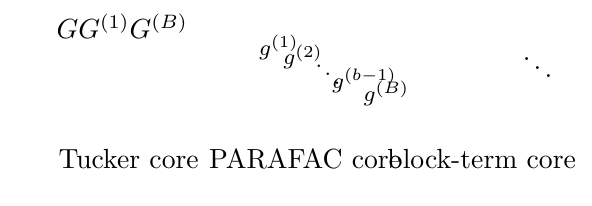
\begin{tikzpicture}[x=\textwidth/14.2, y=-\textwidth/14.2, scale=0.75]
	%\useasboundingbox (0,-1) rectangle (13,3.5);
	\TensorThree{$\ten{G}$}{}{}{}{2}{2}{2}
	\node[anchor=north, align=center] at (1,2) {Tucker core};

	{\footnotesize
	\begin{scope}[shift={(3.5,0)}]
		\TensorThree{}{}{}{}{2}{2}{2}
		\node at (.33,.33,-.33) {$g^{(1)}$};
		\node at (.66,.66,-.66) {$g^{(2)}$};
		\node at (1,1,-1) {$\ddots$};
		\node at (1.5, 1.5, -1.5) {$g^{(b-1)}$};
		\node at (1.8, 1.9, -1.8) {$g^{(B)}$};
	\end{scope}
	}
	\node[anchor=north, align=center] at (4.5,2) {PARAFAC core};

	\begin{scope}[shift={(7,0)}]
		\TensorThree{}{}{}{}{2}{2}{2}
		\TensorThree{$\ten{G}^{(1)}$}{}{}{}{.5}{.5}{.5}
		\node at (.75,.75,-.75) {$\ddots$};
		\begin{scope}[shift={(1,1,-1)}]
			\TensorThree{$\ten{G}^{(B)}$}{}{}{}{1}{1}{1}
		\end{scope}
	\end{scope}
	\node[anchor=north, align=center] at (8,2) {block-term core};
\end{tikzpicture}
